
%% Beginning of file 'sample63.tex'
%%
%% Modified 2019 June
%%
%% This is a sample manuscript marked up using the
%% AASTeX v6.3 LaTeX 2e macros.
%%
%% AASTeX is now based on Alexey Vikhlinin's emulateapj.cls 
%% (Copyright 2000-2015).  See the classfile for details.

%% AASTeX requires revtex4-1.cls (http://publish.aps.org/revtex4/) and
%% other external packages (latexsym, graphicx, amssymb, longtable, and epsf).
%% All of these external packages should already be present in the modern TeX 
%% distributions.  If not they can also be obtained at www.ctan.org.

%% The first piece of markup in an AASTeX v6.x document is the \documentclass
%% command. LaTeX will ignore any data that comes before this command. The 
%% documentclass can take an optional argument to modify the output style.
%% The command below calls the preprint style which will produce a tightly 
%% typeset, one-column, single-spaced document.  It is the default and thus
%% does not need to be explicitly stated.
%%
%%
%% using aastex version 6.3
\documentclass{aastex63}
\usepackage{amsmath}
\usepackage[utf8]{inputenc}
\usepackage{listings}  % for code in latex
\usepackage{color}
% \usepackage{caption}

%% The default is a single spaced, 10 point font, single spaced article.
%% There are 5 other style options available via an optional argument. They
%% can be invoked like this:
%%
%% \documentclass[arguments]{aastex63}
%% 
%% where the layout options are:
%%
%%  twocolumn   : two text columns, 10 point font, single spaced article.
%%                This is the most compact and represent the final published
%%                derived PDF copy of the accepted manuscript from the publisher
%%  manuscript  : one text column, 12 point font, double spaced article.
%%  preprint    : one text column, 12 point font, single spaced article.  
%%  preprint2   : two text columns, 12 point font, single spaced article.
%%  modern      : a stylish, single text column, 12 point font, article with
%% 		  wider left and right margins. This uses the Daniel
%% 		  Foreman-Mackey and David Hogg design.
%%  RNAAS       : Preferred style for Research Notes which are by design 
%%                lacking an abstract and brief. DO NOT use \begin{abstract}
%%                and \end{abstract} with this style.
%%
%% Note that you can submit to the AAS Journals in any of these 6 styles.
%%
%% There are other optional arguments one can invoke to allow other stylistic
%% actions. The available options are:
%%
%%   astrosymb    : Loads Astrosymb font and define \astrocommands. 
%%   tighten      : Makes baselineskip slightly smaller, only works with 
%%                  the twocolumn substyle.
%%   times        : uses times font instead of the default
%%   linenumbers  : turn on lineno package.
%%   trackchanges : required to see the revision mark up and print its output
%%   longauthor   : Do not use the more compressed footnote style (default) for 
%%                  the author/collaboration/affiliations. Instead print all
%%                  affiliation information after each name. Creates a much 
%%                  longer author list but may be desirable for short 
%%                  author papers.
%% twocolappendix : make 2 column appendix.
%%   anonymous    : Do not show the authors, affiliations and acknowledgments 
%%                  for dual anonymous review.
%%
%% these can be used in any combination, e.g.
%%
%% \documentclass[twocolumn,linenumbers,trackchanges]{aastex63}
%%
%% AASTeX v6.* now includes \hyperref support. While we have built in specific
%% defaults into the classfile you can manually override them with the
%% \hypersetup command. For example,
%%
%% \hypersetup{linkcolor=red,citecolor=green,filecolor=cyan,urlcolor=magenta}
%%
%% will change the color of the internal links to red, the links to the
%% bibliography to green, the file links to cyan, and the external links to
%% magenta. Additional information on \hyperref options can be found here:
%% https://www.tug.org/applications/hyperref/manual.html#x1-40003
%%
%% Note that in v6.3 "bookmarks" has been changed to "true" in hyperref
%% to improve the accessibility of the compiled pdf file.
%%
%% If you want to create your own macros, you can do so
%% using \newcommand. Your macros should appear before
%% the \begin{document} command.
%%
\newcommand{\vdag}{(v)^\dagger}
\newcommand\aastex{AAS\TeX}
\newcommand\latex{La\TeX}


%% Reintroduced the \received and \accepted commands from AASTeX v5.2
\received{June 1, 2019}
\revised{January 10, 2019}
\accepted{\today}
%% Command to document which AAS Journal the manuscript was submitted to.
%% Adds "Submitted to " the argument.
\submitjournal{ApJ}

%% For manuscript that include authors in collaborations, AASTeX v6.3
%% builds on the \collaboration command to allow greater freedom to 
%% keep the traditional author+affiliation information but only show
%% subsets. The \collaboration command now must appear AFTER the group
%% of authors in the collaboration and it takes TWO arguments. The last
%% is still the collaboration identifier. The text given in this
%% argument is what will be shown in the manuscript. The first argument
%% is the number of author above the \collaboration command to show with
%% the collaboration text. If there are authors that are not part of any
%% collaboration the \nocollaboration command is used. This command takes
%% one argument which is also the number of authors above to show. A
%% dashed line is shown to indicate no collaboration. This example manuscript
%% shows how these commands work to display specific set of authors 
%% on the front page.
%%
%% For manuscript without any need to use \collaboration the 
%% \AuthorCollaborationLimit command from v6.2 can still be used to 
%% show a subset of authors.
%
%\AuthorCollaborationLimit=2
%
%% will only show Schwarz & Muench on the front page of the manuscript
%% (assuming the \collaboration and \nocollaboration commands are
%% commented out).
%%
%% Note that all of the author will be shown in the published article.
%% This feature is meant to be used prior to acceptance to make the
%% front end of a long author article more manageable. Please do not use
%% this functionality for manuscripts with less than 20 authors. Conversely,
%% please do use this when the number of authors exceeds 40.
%%
%% Use \allauthors at the manuscript end to show the full author list.
%% This command should only be used with \AuthorCollaborationLimit is used.

%% The following command can be used to set the latex table counters.  It
%% is needed in this document because it uses a mix of latex tabular and
%% AASTeX deluxetables.  In general it should not be needed.
%\setcounter{table}{1}

%%%%%%%%%%%%%%%%%%%%%%%%%%%%%%%%%%%%%%%%%%%%%%%%%%%%%%%%%%%%%%%%%%%%%%%%%%%%%%%%
%%
%% The following section outlines numerous optional output that
%% can be displayed in the front matter or as running meta-data.
%%
%% If you wish, you may supply running head information, although
%% this information may be modified by the editorial offices.
\shorttitle{EinsteinPy: Python for General Relativity}
\shortauthors{The EinsteinPy Community}
%%
%% You can add a light gray and diagonal water-mark to the first page 
%% with this command:
%% \watermark{text}
%% where "text", e.g. DRAFT, is the text to appear.  If the text is 
%% long you can control the water-mark size with:
%% \setwatermarkfontsize{dimension}
%% where dimension is any recognized LaTeX dimension, e.g. pt, in, etc.
%%
%%%%%%%%%%%%%%%%%%%%%%%%%%%%%%%%%%%%%%%%%%%%%%%%%%%%%%%%%%%%%%%%%%%%%%%%%%%%%%%%
\graphicspath{{./}{figures/}}
%% This is the end of the preamble.  Indicate the beginning of the
%% manuscript itself with \begin{document}.

\begin{document}

\title{EinsteinPy: Python for General Relativity\footnote{Released on July, 15th, 2019}}

%% LaTeX will automatically break titles if they run longer than
%% one line. However, you may use \\ to force a line break if
%% you desire. In v6.3 you can include a footnote in the title.

%% A significant change from earlier AASTEX versions is in the structure for 
%% calling author and affiliations. The change was necessary to implement 
%% auto-indexing of affiliations which prior was a manual process that could 
%% easily be tedious in large author manuscripts.
%%
%% The \author command is the same as before except it now takes an optional
%% argument which is the 16 digit ORCID. The syntax is:
%% \author[xxxx-xxxx-xxxx-xxxx]{Author Name}
%%
%% This will hyperlink the author name to the author's ORCID page. Note that
%% during compilation, LaTeX will do some limited checking of the format of
%% the ID to make sure it is valid. If the "orcid-ID.png" image file is 
%% present or in the LaTeX pathway, the OrcID icon will appear next to
%% the authors name.
%%
%% Use \affiliation for affiliation information. The old \affil is now aliased
%% to \affiliation. AASTeX v6.3 will automatically index these in the header.
%% When a duplicate is found its index will be the same as its previous entry.
%%
%% Note that \altaffilmark and \altaffiltext have been removed and thus 
%% can not be used to document secondary affiliations. If they are used latex
%% will issue a specific error message and quit. Please use multiple 
%% \affiliation calls for to document more than one affiliation.
%%
%% The new \altaffiliation can be used to indicate some secondary information
%% such as fellowships. This command produces a non-numeric footnote that is
%% set away from the numeric \affiliation footnotes.  NOTE that if an
%% \altaffiliation command is used it must come BEFORE the \affiliation call,
%% right after the \author command, in order to place the footnotes in
%% the proper location.
%%
%% Use \email to set provide email addresses. Each \email will appear on its
%% own line so you can put multiple email address in one \email call. A new
%% \correspondingauthor command is available in V6.3 to identify the
%% corresponding author of the manuscript. It is the author's responsibility
%% to make sure this name is also in the author list.
%%
%% While authors can be grouped inside the same \author and \affiliation
%% commands it is better to have a single author for each. This allows for
%% one to exploit all the new benefits and should make book-keeping easier.
%%
%% If done correctly the peer review system will be able to
%% automatically put the author and affiliation information from the manuscript
%% and save the corresponding author the trouble of entering it by hand.
\newcommand{\sceeiitmandi}{School of Computing and Electrical Engineering, Indian Institute of Technology Mandi, India}

% \author[0000-0000-0000-0000]{The SunPy Community}
% \noaffiliation

% \author[orcid-id]{name}
% \affiliation{}
% below add contributing authors (those folks that have actually worked writing the paper).
% board members get some symbol next to their names.

\author[0000-0002-0870-4665]{Shreyas Bapat}
\altaffiliation{EinsteinPy Lead Developer, EinsteinPy Board Member}
\affiliation{\sceeiitmandi}

\author[0000-0002-1900-3338]{Shilpi Jain}
\altaffiliation{EinsteinPy Board Member}
\affiliation{Department of Earth Sciences, Indian Institute of Technology Roorkee, India}

\author[0000-0002-2369-0628]{Ritwik Saha}
\altaffiliation{EinsteinPy Lead Developer, EinsteinPy Board Member}
\affiliation{\sceeiitmandi}

\author[0000-0002-2784-5666]{Bhavya Bhatt}
\altaffiliation{EinsteinPy Deputy Lead Developer}
\affiliation{\sceeiitmandi}

\author[0000-0003-3354-1893]{Akshita Jain}
\affiliation{\sceeiitmandi}

\collaboration{1000}{(Primary Paper Contributors)}

% Below add contributors to the Sunpy project
% this list is ordered alphabetically

\author[0000-0003-1021-3336]{Priyanshu Khandelwal}
\altaffiliation{EinsteinPy Board Member}
\affiliation{\sceeiitmandi}

\author[0000-0002-1928-1549]{Rishi Sharma}
\altaffiliation{EinsteinPy Board Member}
\affiliation{\sceeiitmandi}

\author[0000-0002-2268-9772]{Sofía Ortín Vela}
\affil{University of Zaragoza, Spain}

\author[0000-0001-8530-7252]{Jialin Ma}
\affil{Georgia Institute of Technology, USA}

\author[0000-0001-7234-6148]{Varun Singh}
\affiliation{\sceeiitmandi}

\author[0000-0002-7179-3795]{Alpesh Jamgade}
\affiliation{Department of Mathematics, Bharath Institute of Higher Education and Research, Chennai, India}

\author[0000-0002-5198-9010]{Manvi Gupta}
\affiliation{\sceeiitmandi}

\author{Tushar Tyagi}
\affiliation{\sceeiitmandi}

\author[0000-0003-4387-8078]{Divya Gupta}
\affiliation{\sceeiitmandi}

\author{Hrishikesh Sudam Sarode}
\affiliation{\sceeiitmandi}

\author[0000-0003-1838-8368]{Tanmay Rustagi}
\affiliation{\sceeiitmandi}

\author[0000-0002-0757-2883]{Abhijeet Manhas}
\affiliation{\sceeiitmandi}

\author[0000-0001-5558-9447]{Raphael Reyna}
\affiliation{California State Polytechnic University, Pomona, USA}

\author[0000-0002-6696-8730]{Govind Dixit}
\affiliation{Information Technology, Indian Institute of Information Technology Lucknow, India}

\author{Ratin Kumar}
\affiliation{National Institute of Technology Kurukshetra, India}

\author[0000-0001-8302-1584]{Sashank Mishra}
\affiliation{Department of Information Technology, Indian Institute of Information Technology Allahabad, India}

\author[0000-0003-0973-4994]{Pratyush Kerhalkar}
\affiliation{Department of Electronics and Communication Engineering, Manipal Institute of Technology, India}

\collaboration{1000}{(EinsteinPy Contributors)}

\correspondingauthor{Shreyas Bapat}
\email{shreyas@einsteinpy.org, bapat.shreyas@gmail.com}



%% Note that the \and command from previous versions of AASTeX is now
%% depreciated in this version as it is no longer necessary. AASTeX 
%% automatically takes care of all commas and "and"s between authors names.

%% AASTeX 6.3 has the new \collaboration and \nocollaboration commands to
%% provide the collaboration status of a group of authors. These commands 
%% can be used either before or after the list of corresponding authors. The
%% argument for \collaboration is the collaboration identifier. Authors are
%% encouraged to surround collaboration identifiers with ()s. The 
%% \nocollaboration command takes no argument and exists to indicate that
%% the nearby authors are not part of surrounding collaborations.

%% Mark off the abstract in the ``abstract'' environment. 
\begin{abstract}

This paper presents EinsteinPy (version 0.3), a community-developed Python
package for gravitational and relativistic astrophysics. Python is a free, easy to use high level programming language which has seen a huge expansion in the number of its users and developers in recent years. Specifically, a lot of recent studies show that the use of Python in Astrophysics and in general physics has increased exponentially. Many great frameworks came as Python packages which provide a very high level of abstraction over the dirty nitty-gritty of complex algorithms and provide an easy to use interfaceand pleasing user experience. One such example is Keras - framework for deep learning which has made deep learning so easy that a person with zero programming knowledge can also train a neural network classifier. This example really demonstrates the power of abstraction which is achievable in Python. The aim of the EinsteinPy is no different and is developed keeping in mind the state of a theoretical gravitational physicist with a little or no background in computer programming and trying to work in the field of numerical relativity or trying to use simulations in their research. Currently EinsteinPy supports simulation of time-like and null geodesics and calculate trajectories in different background geometries some of which are Schwarzschild, Kerr and KerrNewmann along with coordinate inter-conversion pipeline. It has a partially developed pipeline for plotting and visualization with dependencies on libraries like plotly, matplotlib etc. One of the unique feature of EinsteinPy is a sufficiently developed symbolic tensor manipulation utilites which is a great tool in itself for teaching yourself tensor algebra which for many beginner students can be overwhelmingly tricky. Currently EinsteinPy also provide few utility functions for hypersurface embedding of Schwarzschild spacetime which further will be extended to model gravitational lensing simulation. The current version of the library is in a state that can be used by any serious student of general relativity trying to get essence of this beautiful subject but is somewhere lost in the heavy mathematical formalism of the subject. EinsteinPy provides such students to really see through the equations and visualize whats really happening.



\end{abstract}

%% Keywords should appear after the \end{abstract} command. 
%% See the online documentation for the full list of available subject
%% keywords and the rules for their use.
\keywords{gravitational physics, astrophysics --- 
simulations --- black holes --- gravitational waves}


%% From the front matter, we move on to the body of the paper.
%% Sections are demarcated by \section and \subsection, respectively.
%% Observe the use of the LaTeX \label
%% command after the \subsection to give a symbolic KEY to the
%% subsection for cross-referencing in a \ref command.
%% You can use LaTeX's \ref and \label commands to keep track of
%% cross-references to sections, equations, tables, and figures.
%% That way, if you change the order of any elements, LaTeX will
%% automatically renumber them.
%%
%% We recommend that authors also use the natbib \citep
%% and \citet commands to identify citations.  The citations are
%% tied to the reference list via symbolic KEYs. The KEY corresponds
%% to the KEY in the \bibitem in the reference list below. 



\section{Introduction} \label{sec:intro}
The relativistic theory of gravity paved its way to the ground in 1915?, when Prof. Albert Einstein published his paper on the general theory of relativity. This elegant and rigorous framework was a generalized version of gravity-free theory - special relativity, which he published earlier in 1905. Almost a hundred years after Einstein wrote down the equations of General Relativity, solutions of the Einstein field equations remain extremely difficult to find beyond those which exhibit significant symmetries.\\
We can study the behavior of solutions under a high degree of symmetry considerations and could even solve analytically for highly unrealistic systems. In case of problems relevant to astrophysical and gravitational physics research, it still remains a big daunting question on how to get around the problem of solving these field equations. This question is so profound that it has a separate profound field of research which goes with the name of numerical relativity which attempts to use computation science and programming to numerically obtain solutions of the equations (which would be the background geometry) for some turbulent region where most of the interesting dynamics are happening (as we can not solve for an infinitely large grid due to restrictions imposed on us by space and time complexity and computability).\\
Numerical methods have been used to solve the Einstein equation for many decades, but the past decade has seen tremendous advances and adding to that, the interest of the community grew when the field found applications in areas of radio astronomy, cosmology, signal processing, data mining. The field of numerical relativity is growing rampantly with the vast literature on algorithms, numerical methods and theoretical formulations (from basic 3+1 decomposition formulation to more sophisticated ones) with the development of robust and involved frameworks that provide a complete programming ecosystem and have proved to be essential tools for any numerical relativity researcher.\\
Reflecting the other end of the research community stands the major section of theoretical physicists which counts the majority as a novice in programming. The head challenge is the fact that the usage of these frameworks demands heavy use of high-level programming languages like C, C++, Python, etc. Though Python provides a vast room for abstractions no library existed that focused towards numerical relativity, eventually, the need of python library dedicated to general relativity became the propellant for the team and thus they made dauntless efforts to cover the space for this Python library. Since then, EinsteinPy has seen a lot of contributions from people all over the world and many ”good to go” functionalities are already provided in this and previous versions.\\
EinsteinPy is made to provide a set of tools which can make numerical computations for solving Einstein’s field equations an easy job for anyone who does not want to deal with intricacies of the subject along with few, very basic but powerful functionalities that could be used by anyone who wants to learn the subject of general relativity with every minute detail.
The library is as an attempt to provide programming and numerical environment for numerous numerical relativity problems like geodesics plotter, gravitational lensing and ray tracing, solving and simulating relativistic hydrodynamical equations, plotting of black hole event horizons, solving Einstein’s field equations and simulating various dynamical systems like binary merger etc.\\
EinsteinPy provides an open-source and open-development core package and aims to build an ecosystem of affiliated packages that support numeric relativity functionality in the Python programming language. ”Open development” describes a process where anybody with an internet connection can suggest changes to the source code and contribute their opinion when new features, bug fixes or other code changes, governance, or any other aspect of the development process is discussed. EinsteinPy core package is now a feature-rich library of sufficiently general tools and classes that support the development of more specialized code\\
In the further coming section, we discuss with some of the features of the current as well previous version and the future plans which are yet to be implemented in the upcoming versions.Also, we describe a few code snippets to explain the usage of the library on which more details can be found on the organization website. The development of the EinsteinPy core package began as a community-driven effort to standardize core functionality for software in Python which renders a user-friendly interface for supporting numerical relativity and relativistic astrophysics research.\\
We start this paper by describing the way EinsteinPy functions followed by the main software efforts developed by the EinsteinPy itself with proper detailed documentation of the current version release. We end with a short vision for the future of EinsteinPy to its contribution in the field of computational methodology in gravitational and relativistic Astrophysics.


\section{Data Types} \label{sec:datatypes}

The EinsteinPy package provides some core data types for calculating, operating on, visualizing geodesics and black holes. There are some data types created for symbolic manipulations and calculations of relativistic tensors. The most important data types for EinsteinPy are \texttt{Body}, \texttt{Geodesic} and \texttt{BaseRelativityTensor} objects that support defining and creating new bodies, storing and calculating geodesic for bodies, and handling respectively. The main purpose of these core classes is to standardize the way calculations and visualizations are done for various kinds of heavy cosmic bodies and black holes. The classes always maintain the consistency in units of measurement wherever applicable, and create a consistent and clean API for any non-programmer to understand. The classes are designed such that it resembles the flow of physics and are  as intuitional as possible. These core classes also include a rigid architecture for data manipulation and visualizations wherever applicable. Following sections provide deep insight into the above mentioned three code data types of EinsteinPy:

\subsection{Body} \label{subsec:Body}
The Body data type helps define the central black-hole or the heavy massed object and the objects revolving around it. A new body can be defined by some of the very basic constraints:

\begin{itemize}
\item \texttt{name}: Body Name,
\item \texttt{mass}: Mass of the body with attached astropy units 
\item \texttt{R}: Radius of the body with attached astropy units
\item \texttt{differential}: Complete position and velocity vector of the body in form of a Cartesian / Spherical / BoyerLindquist data class object from einsteinpy coordinates (optional)
\item \texttt{a}: Spin factor (a) of the body for Kerr Solutions with attached astropy units (optional)
\item \texttt{q}: Charge of the body with attached astropy units (optional)
\item \texttt{is\_attractor}: A boolean variable concerned with if the body is to be supposed as a central attractor. (optional)
\item \texttt{parent}: Parent body for the body, object of the same data class (optional)
\end{itemize}

\subsection{Geodesic} \label{subsec:Geodesic}
The Body data type helps define the central black-hole or the heavy massed object and the objects revolving around it. A new body can be defined by some of the very basic constraints:

\subsection{BaseRelativityTensor} \label{subsec:BaseRelativityTensor}
This is a base class from which other tensors in \textit{symbolic} module are derived. The user can use this class to create his/her own tensor while using the various in-built functions provided by this class. The class also maintains the indicial configuration of the tensor(contravariant and covariant indices), calculates the free variables used in describing the tensor other than those which depicts the axis of space-time itself (e.g. $t, x, y, z$). The class has a function to convert the symbolic tensorial quantities into functions where actual numerical values can be substitued.

This class along with its parent class \textit{Tensor} have the following functions/properties,
\begin{itemize}
\item \texttt{order} (Property) : Returns the order of the tensor. 
\item \texttt{config} (Property) : Returns the arrangement of contravariant(upper)/covariant(lower) indices of the tensor. For example, 'ulll'.
\item \texttt{parent\_metric} (Property) : Returns the metric tensor of the space-time associated with the tensor, if present. Else returns \texttt{None}.
\item \texttt{tensor} (Function) : Returns the tensorial quantity contained within the class instance.
\item \texttt{subs} (Function) : Returns a new tensor upon substitution of current variables with new variables/values.
\item \texttt{simplify} (Function) : Returns a tensor contain simplified expressions from the current tensor.
\item \texttt{symbols} (Function) : Returns the symbols denoting each axis of the space-time.
\item \texttt{tensor\_lambdify} (Function) : Returns lambdified function of symbolic tensors. This means that the returned functions can accept numerical values and return numerical quantities.
\item \texttt{lorentz\_transform} (Function) : Returns a lorentz-transformed tensor when supplied with a transformation matrix. This function also considers the contravariance and covariance of tensors during transformation.
\end{itemize}


\section{UNIT HANDLING} \label{sec:unithandle}
All user-facing functionality provided by einsteinpy make use of astropy.units. 
All functions and objects must have their input constrained to the appropriate type of unit (e.g., length, mass or energy). Inputs can then be provided with any units that match the required type (e.g., millimeters and inches are both valid units for length) and conversions occur automatically without user intervention. The einsteinpy.constant subpackage contains a few standard constants.

\section{Development Model} \label{sec:devmodels}
The EinsteinPy Project follows an open development model, which is widely used in the scientific Python community and other computational astrophysics packages. The project is hosted on GitHub as a public repository with restricted write access to some key people. Anyone, however is welcome and encouraged to make code contributions and suggest changes using pull requests. Since the repository containing the codebase is licenced under an open and permissive MIT licence,  the project allows commercial use, modification, sublicensing, distribution and private use as long as the copyright notice and licence is redistributed. The project uses git for distributed version control and relies on CircleCI, Codefactor, GitHub Actions etc. for running the unit tests and other CI checks for every pull request.
The code quality is maintained at the highest standards with strong control on the cyclomatic complexity, code linting, imports ordering and a proper docstring wherever necessary. Every contribution is reviewed and it must meet the following requirements: 

\begin{itemize}
\item \texttt The code must strictly adhere to the PEP8 Standards, on the top of it, the code must be linted with black to save the reviewer’s time identifying the changes made and reduce the diff generated because of the patch.
\item \texttt The imports in the code must be sorted using tools such as isort. 
\item \texttt The documentation follows numpy like docstrings, and a proper reStructured Text syntax is followed for writing the documentation.
\item \texttt The changelog is populated at release-time by the lead developer and the releasing developer
\end{itemize}
EinsteinPy further follows a trunk-based development model, which ensures a new branch for every minor release and new patch release made using the minor release branch. All the latest changes are kept on the master branch on GitHub and the relevant issues are closed as soon as the pull request solving it merges onto the master. A release having the changes is made at a later date. 
EinsteinPy only supports the latest bleeding-edge Python, Numpy and Astropy versions.  All the stable Python versions after Python 3.5 are supported. All the code snippets written follow the guidelines of numba in order to accelerate the Python code and make the simulations faster. 




\section{The EinsteinPy Core Package} \label{sec:core}
This section explains in detail, the modules available within EinsteinPy core pacakge, their API and the purpose they serve.
\subsection{METRIC} \label{subsec:metric}
This module captures all the geometric and causal structure of specific spacetimes, and being able to calculate trajectories in a given space-time. 
The module derives its name from Metric Tensor, a tensorial quantity used to describe differential lengths, especially in a curved space-time. 
However, this module serves more than its usual definition and ultimately leads us to obtain geodesics of particles in a spacetime with high curvature, where notions of newtonian physics fail.
\subsubsection{Schwarzschild Metric} \label{subsubsec:sch}
Karl Schwarzchild pioneered the analysis of the relation between the size of black hole and its mass and this work paved the way for the first exact solution of Einstein's Field Equation under the limited case of single spherical non-rotating, non-charged body. 
The metric equation corrosponding to a space-time centred around a body in the above described conditions is given by,

\begin{align}
& ds^2 = -c^2 d\tau ^2 = - (1 - \frac{r_s}{r})c^2 dt^2  + \frac{1}{(1 - \frac{r_s}{r})}dr^2 + r^2 d\theta ^2 + r^2 sin^2 \theta d\phi ^2
\end{align}

The same equation can be written in a tensorial form as follows,

\begin{gather}
g_{\mu \nu} = \begin{bmatrix} - (1 - \frac{r_s}{r})c^2 & 0 & 0 & 0 \\ 0 & \frac{1}{(1 - \frac{r_s}{r})} & 0 & 0 \\ 0 & 0 & r^2 & 0 \\ 0 & 0 & 0 &  r^2 sin^2 \theta \end{bmatrix} \\ 
\nonumber \\
ds^2 = g_{\mu \nu} dx^\mu dx^\nu
\end{gather}

where $r_s$ is the schwarzschild radius of a given heavy body and is given by the equation,

\begin{gather}
r_s = \frac{2GM}{c^2}
\end{gather}

$G$, $M$, and $c$ are gravitational constant, mass of the body and speed of light in vacuum respectively.

Schwarzschild Radius is a limit below which the degree of space-time curvature causes the partcle to undergo irreversible gravitational collapse wherein the partcle would need a speed greater than speed of light ot escape singularity.

As $r \to \infty$, the metric defined above starts to approximate flat Minkowski space-time, thus showing that Schwarzschild geometry is asymptotically flat. 

If supplied with initial position and velocity of a particle with negligible mass(in comparision to the central body), we can obtain the geodesics of the particle for a given range of proper time $\tau$, as it boils down to a set of eight differential equations numerically solvable by a class of Runge-Kutta methods.

The file \textbf{schwarzschild.py} contains the class \textit{Schwarzschild} for defining Schwarzschild geometry methods.

Here is a working code describing the motion of particle revolving around a black hole of mass approximately equal to mass of the Earth. As the trajectory starts from a mere $130m$ from the black hole, we obtain some interesting observations.

\begin{lstlisting}[language=Python, caption=Importing the required modules]
>>> import numpy as np
>>> import astropy.units as u
>>> from einsteinpy.plotting import GeodesicPlotter
>>> from einsteinpy.coordinates import SphericalDifferential
>>> from einsteinpy.bodies import Body
>>> from einsteinpy.geodesic import Geodesic
>>> from einsteinpy.metric import Schwarzschild
\end{lstlisting}

\begin{lstlisting}[language=Python, caption=Defining the attractor and the particle and calculating geodesics]
>>> Attractor = Body(name="BH", mass=6e24 * u.kg)
>>> init_conditions = SphericalDifferential(130*u.m, np.pi/2*u.rad, -np.pi/8*u.rad,
...                                         0*u.m/u.s, 0*u.rad/u.s, 1900*u.rad/u.s)
>>> Particle = Body(differential=init_conditions, parent=Attractor)
>>> geodesic = Geodesic(body=Particle, time=0 * u.s, end_lambda=0.00205, step_size=5e-8,
...                     metric=Schwarzschild)
>>> geodesic.trajectory
array([[ 0.00000000e+00,  1.20104339e+02, -4.97488462e+01, ...,
         9.45228078e+04,  2.28198245e+05,  0.00000000e+00],
       [ 3.99986427e-08,  1.20108103e+02, -4.97397110e+01, ...,
         9.36472607e+04,  2.28560869e+05, -5.80280784e-14],
       ...,
       [ 2.04962579e-03,  1.04114904e+02,  1.08255773e+01, ...,
        -1.23245830e+06,  1.80261847e+05, -9.67931265e-09],
       [ 2.05002578e-03,  1.03619005e+02,  1.08973776e+01, ...,
        -1.24706334e+06,  1.78734562e+05, -9.79337222e-09]])
>>> geodesic.trajectory.shape
(6567, 8)
\end{lstlisting}
We can see that for each timestep, we obtain eight values : $t$, $r$, $\theta$, $\phi$, $v_t$, $v_r$, $v_\theta$ and $v_\phi$ corrosponding to coordinate time, radial distance from the centre, polar angle, azimuth angle and their respective velocities w.r.t proper time $\tau$.

Further, we plot the trajectory in 2D for vizualization purposes.
\begin{lstlisting}[language=Python, caption=Plotting the trajectory]
>>> obj = GeodesicPlotter()
>>> obj.plot(geodesic)
>>> obj.show()
\end{lstlisting}

\begin{figure}[h]
	\centering
	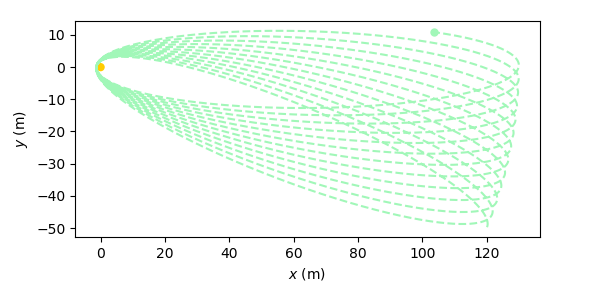
\includegraphics[scale=0.7]{images/perihelion_cropped.png}
	%\centerline{\includegraphics{ftcbuild2.pdf}}
	\caption{Plot obtained from the above code showing the phenomenon of perihelion advance}
	\label{fig:schwarzschild}
\end{figure}

We observe the phenomenon of perihelion advance of a particle around a heavy body due to spacetime curavture. The orbit would have been purely eliptical if plotted in accordance with Newtonian Mechanics, however, the curvature of space-time around the heavy mass shifts the orbit with each revolution. In practicality, this phenomenon is not so pronounced as no particle approaches a heavy mass this closely. For instance, Mercury advances its perihelion at a rate of $42.98\pm 0.04$ arcsec/century.

\subsubsection{Kerr Metric}\label{subsubsec:kerr}
Kerr metric is a further generalization of Schwarzschild metric and a specific case of Kerr-Newman geometry. A spacetime is defined as a "Kerr" spacetime as and when the massive central body posseses an angular momentum. The corresponding metric equation which defines the space-time is,

\begin{gather}
g_{\mu \nu} = \begin{bmatrix} - (1 - \frac{r_s r}{\Sigma})c^2 & 0 & 0 & -\frac{r_s r a sin^2 \theta}{\Sigma}c \\ 0 & \frac{\Sigma}{\Delta} & 0 & 0 \\ 0 & 0 & \Sigma & 0 \\ -\frac{r_s r a sin^2 \theta}{\Sigma}c & 0 & 0 &  (r^2 + a^2 + \frac{r_s r a^2}{\Sigma}sin^2 \theta) sin^2 \theta \end{bmatrix} \\ 
\nonumber \\
ds^2 = g_{\mu \nu} dx^\mu dx^\nu
\end{gather}

where,
\begin{gather}
a = \frac{J}{Mc}, \nonumber \\
\Sigma = r^2 + a^2 cos^2, \nonumber \theta \\
\Delta  = r^2 - r_s r + a^2 \nonumber
\end{gather}

$J$ is the angular momentum of the body and all the other symbols hold their usual meanings as discussed in \ref{subsubsec:sch}. The coordinate system used to describe the metric is Boyer-Lindquist coordinate system.

The file \textbf{kerr.py} contains the class \textit{Kerr} for defining Schwarzschild geometry methods.

APIs for \textit{Schwarzschild}, \textit{Kerr} and \textit{KerrNewman} are consistent and code structure remains same for the sake for clarity and intuitiveness. For example,

\begin{lstlisting}[language=Python, caption=Defining the Kerr Body and the particle and calculating geodesics]
>>> a = 0.3 * u.m
>>> Attractor = Body(name="BH", mass=1.989e30 * u.kg, a=a)
>>> init_conditions = BoyerLindquistDifferential(49.95e5 * u.km, np.pi / 2 * u.rad, 
...                                              np.pi * u.rad, 0 * u.km / u.s, 
...                                              0 * u.rad / u.s, 0 * u.rad / u.s,
...                                              a)
>>> Particle = Body(differential=init_conditions, parent=Attractor)
>>> geodesic = Geodesic(body=Particle, time=0 * u.s, end_lambda=33932.90,
...                     step_size=1.2, metric=Kerr)
\end{lstlisting}

As evident from the code, API across different classes are made to be as homegenous as possible.

As a rotating black hole drags the space-time around it, a freely falling object acquires a angular velocity around the coordinate centre, i.e centre of the black hole. This effect is evident from the plot obatined from the above geodesics, in the same way as obtained one in the Schwarzschild example.

\begin{figure}[h]
	\centering
	
\includegraphics[scale=0.1]{images/blank.jpg} %replace this when the actual plot becomes available
	%\centerline{\includegraphics{ftcbuild2.pdf}}
	\caption{Plot obtained from the above geodesics showing the phenomenon of frame dragging}
	\label{fig:kerr}
\end{figure}


\subsubsection{Kerr-Newman Metric}\label{subsubsec:kerrnewman}
Kerr-Newman metric presents the most general case within single-body vacuum solutions of Einstein Field Equation. It generalizes all the quantities used to describe a black hole, as affirmed by "no hair" theoram, i.e. Charge $Q$, Angular Momentum $J$ and Mass $M$. The metric equation is given by,

\begin{gather}
-ds^2 = c^2 d\tau^2 = -(\frac{dr^2}{\Delta}+d\theta^2)\rho^2 + (c dt - a sin^2 \theta d\phi)^2 \frac{\Delta}{\rho^2} - ((r^2 + a^2)d\phi - ac dt)^2 \frac{sin^2 \theta}{\rho^2}
\end{gather}

where,

\begin{gather}
a = \frac{J}{Mc}, \nonumber \\
\Sigma = r^2 + a^2 cos^2 \theta , \nonumber  \\
\Delta  = r^2 - r_s r + a^2 + r_Q ^ 2, \nonumber \\
r_Q ^ 2 = \frac{Q^2 G}{4\pi\epsilon_0 c^4} \nonumber
\end{gather}

All the other symbols convey their usual meanings, as discussed in the previous two sections \ref{subsubsec:sch} and \ref{subsubsec:kerr}. For the sake of brevity, we would not go into the specifics of this class as the classes within \textit{Metric} module share very similar APIs as inferred in \ref{subsubsec:kerr}.

\subsection{COORDINATES}
\subsection{SYMBOLIC}
General Relativity required heavy mathematical formulation to derive and describe various tensors attributing to various features essential for cogent description of a arbitrary space-time. We would describe the various quantities currently supported by this module while maintaining brevity. Each quantity has its own class, even scalars, which are treated as 0\textsuperscript{th} order tensors.

All the mathematical quantities build upon \textit{BaseRelativityTensor} as derived classes, which is discussed in detail in \ref{subsec:BaseRelativityTensor}. 

\subsubsection{MetricTensor}\label{subsubsec:metric}
Metric Tensor describes the differential length elements required to measure distance in a curved(also applies to flat) space-time. It is a second order tensor and is fundamental to describe any space-time geometry. The \textit{MetricTensor} class, being inherited from \textit{BaseRelativityTensor} (\ref{subsec:BaseRelativityTensor}) , inherits all its functions and also have some functions and constraints of its own. For example, metric tensor is bound to be a second order tensor.

The defined class functions are :
\begin{itemize}
\item \texttt{change\_config} : returns a different instance of the same class with different index (contravariant or covariant) configuration. 
\item \texttt{inv} : returns inverse of the metric
\end{itemize}

Also, the library maintains an ever expanding predefined metrics for direct use. Here's an code snippet for a better dive into the specificities of the class.

\begin{lstlisting}[language=Python, caption=Importing a predefined metric]
>>> from einsteinpy.symbolic.predefined import CMetric
>>> metric = CMetric
>>> metric.tensor()
\end{lstlisting}

\begin{center}
$\displaystyle \left[\begin{matrix}- \frac{h{\left(y \right)}}{\left(x + y\right)^{2}} & 0 & 0 & 0\\0 & \frac{1}{\left(x + y\right)^{2} f{\left(x \right)}} & 0 & 0\\0 & 0 & \frac{1}{\left(x + y\right)^{2} h{\left(y \right)}} & 0\\0 & 0 & 0 & \frac{f{\left(x \right)}}{\left(x + y\right)^{2}}\end{matrix}\right]$
\end{center}

\begin{lstlisting}[language=Python, caption=Displaying the contravarint configuration of metric]
>>> metric.change_config("uu").tensor()
\end{lstlisting}

\begin{center}
 $\displaystyle \left[\begin{matrix}- \frac{\left(x + y\right)^{2}}{h{\left(y \right)}} & 0 & 0 & 0\\0 & \left(x + y\right)^{2} f{\left(x \right)} & 0 & 0\\0 & 0 & \left(x + y\right)^{2} h{\left(y \right)} & 0\\0 & 0 & 0 & \frac{\left(x + y\right)^{2}}{f{\left(x \right)}}\end{matrix}\right]$ \\
\end{center}

\subsubsection{ChristoffelSymbols}\label{subsubsec:chl}
\subsubsection{RiemannCurvatureTensor}\label{subsubsec:riemann}
\subsubsection{RicciTensor}\label{subsubsec:riccitensor}
\subsubsection{RicciScalar}\label{subsubsec:ricciscalar}
\subsubsection{Other Defined Quantities}\label{subsubsec:other}

\subsection{HYPERSURFACE}
\subsection{PLOTTING}

\section{INFRASTRUCTURE} \label{sec:infra}
\subsection{ Testing} \label{subsec:testing}
The EinsteinPy Project maintains a very high bar in accepting changes and introducing new features. Every patch of code that is accepted in the codebase through any pull request has to be well tested using some unit tests unless given an exception after discussion with both the lead developers. Currently the coverage of unit tests, which means the total fraction of codebase run by at least one unit test is 94\% and we hope to improve it in the future. The 100\% code coverage for this software at this level is not possible because of lack of accurate data to test the code against. We deliberately leave some parts of the codebase out of the testing loop because testing those modules is not possible with the current knowledge level and expertise. However, 94\% code coverage is good enough when we consider other packages in scientific Python community who face the similar problem.  

The test suite can be run manually as well as it runs in an automated fashion on every commit as well as pull request to maintain the code standards, and make it easier for contributors to understand the implications and impact of their changes. The EinsteinPy Project uses many continuous-integration services which provide services to create automated pipelines for code inspection, unit testing, coverage publishing etc. All the contributions trigger these free services (Codecov, CircleCI, Appveyor, GitHub Actions, Codefactor, Codeclimate, Hound, WIP) which are integrated with GitHub repository. All the pull requests are checked for code linting by a pep8speaks bot, which suggests the lines of code which violate the PEP8 standard to the contributor in a human readable way. All these services run on three types of operating systems (Windows, MacOS and Linux). The unit tests run on various versions of Python. They test the documentation builds, test coverage, check whether the pull request author has indicated that it is a work in progress (WIP).They also run several code linting checks which further triggers the unit test build.

\subsection{ Documentation and gallery} \label{subsec:doc}

\section{COMMUNITY} \label{sec:COMMUNITY}
EinsteinPy is being developed as an open source community inside the wide and diverse general scientific python community. Our code is freely available, and we have seen a lot of people contributing and joining us since over the past year.
We touched the landmark of 30 members recently. EinsteinPy is dedicated to problems arising in General Relativity and gravitational physics as well as encouraging open source development. EinsteinPy has benefited greatly from summer of code schemes. Last year EinsteinPy participated in the ESA Summer of Code In Space (SOCIS). This program is inspired by Google Summer Of Code (GSOC) and aims to raise the awareness of open source projects related to space, promote the European Space Agency. The symbolic module in EinsteinPy project was developed during this program.

\section{FUTURE} \label{sec:FUTURE}
We intend to add more functionalities to our project, some of which are, 
\begin{itemize}
\item \texttt Support for null-geodesics in different geometries, . 
\item \texttt Relativistic hydrodynamics
\item \texttt Adaptive Mesh Refinement 
\item \texttt Providing numerical solutions to Einstein’s equations for arbitrarily complex matter distribution.
\end{itemize}

We have an open community where suggestions from people to add functionalities are welcome. We wish to be as helpful as possible to people using EinsteinPy in.



























\acknowledgments

We thank all the people that have made this AASTeX what it is today.  This
includes but not limited to Bob Hanisch, Chris Biemesderfer, Lee Brotzman,
Pierre Landau, Arthur Ogawa, Maxim Markevitch, Alexey Vikhlinin and Amy
Hendrickson. Also special thanks to David Hogg and Daniel Foreman-Mackey
for the new "modern" style design. Considerable help was provided via bug
reports and hacks from numerous people including Patricio Cubillos, Alex
Drlica-Wagner, Sean Lake, Michele Bannister, Peter Williams, and Jonathan
Gagne.

%% To help institutions obtain information on the effectiveness of their 
%% telescopes the AAS Journals has created a group of keywords for telescope 
%% facilities.
%
%% Following the acknowledgments section, use the following syntax and the
%% \facility{} or \facilities{} macros to list the keywords of facilities used 
%% in the research for the paper.  Each keyword is check against the master 
%% list during copy editing.  Individual instruments can be provided in 
%% parentheses, after the keyword, but they are not verified.

\vspace{5mm}
\facilities{HST(STIS), Swift(XRT and UVOT), AAVSO, CTIO:1.3m,
CTIO:1.5m,CXO}

%% Similar to \facility{}, there is the optional \software command to allow 
%% authors a place to specify which programs were used during the creation of 
%% the manuscript. Authors should list each code and include either a
%% citation or url to the code inside ()s when available.

\software{astropy \citep{2013A&A...558A..33A},  
          Cloudy \citep{2013RMxAA..49..137F}, 
          SExtractor \citep{1996A&AS..117..393B}
          }

%% Appendix material should be preceded with a single \appendix command.
%% There should be a \section command for each appendix. Mark appendix
%% subsections with the same markup you use in the main body of the paper.

%% Each Appendix (indicated with \section) will be lettered A, B, C, etc.
%% The equation counter will reset when it encounters the \appendix
%% command and will number appendix equations (A1), (A2), etc. The
%% Figure and Table counter will not reset.

\appendix

\section{Appendix information}

Appendices can be broken into separate sections just like in the main text.
The only difference is that each appendix section is indexed by a letter
(A, B, C, etc.) instead of a number.  Likewise numbered equations have
the section letter appended.  Here is an equation as an example.

\begin{equation}
I = \frac{1}{1 + d_{1}^{P (1 + d_{2} )}}
\end{equation}

Appendix tables and figures should not be numbered like equations. Instead
they should continue the sequence from the main article body.


%% For this sample we use BibTeX plus aasjournals.bst to generate the
%% the bibliography. The sample63.bib file was populated from ADS. To
%% get the citations to show in the compiled file do the following:
%%
%% pdflatex sample63.tex
%% bibtext sample63
%% pdflatex sample63.tex
%% pdflatex sample63.tex

\bibliography{sample63}{}
\bibliographystyle{aasjournal}

%% This command is needed to show the entire author+affiliation list when
%% the collaboration and author truncation commands are used.  It has to
%% go at the end of the manuscript.
%\allauthors

%% Include this line if you are using the \added, \replaced, \deleted
%% commands to see a summary list of all changes at the end of the article.
%\listofchanges
\end{document}

